\begin{opinion}

El trabajo \textbf{``Base de Imágenes Dermatoscópicas Anotadas para el Ecosistema DermaUH: Diseño e
Implementación''} da respuesta a una de las tareas del proyecto ``Desarrollo de aplicaciones basadas
en análisis imagenológico en apoyo al diagnóstico y tratamiento de lesiones cutáneas''. Este proyecto
está asociado al Programa Nacional 6 ``Telecomunicaciones e Informatización de la sociedad''.

Poder contar con una colección de imágenes de pieles cubanas, la primera de este tipo en nuestro país,
constituye un objetivo importante del proyecto. En un contexto donde los repositorios globales
presentan sesgos demográficos que afectan la fiabilidad de la inteligencia artificial en poblaciones
mestizas, este trabajo dota a la dermatología cubana de una herramienta propia capaz de capturar
nuestra diversidad fenotípica, específicamente los \textbf{fototipos III, IV y V}, los cuales están
subrepresentados en la literatura científica internacional.

El autor demuestra un dominio avanzado de la ingeniería de software moderna al adoptar los
principios de la Arquitectura Limpia (Clean Architecture). La implementación sobre la plataforma .NET
10, el uso de C\# 13 y la persistencia en PostgreSQL 17 garantizan un sistema robusto, mantenible y
escalable. Esta separación de responsabilidades en capas permite que el núcleo del negocio
permanezca independiente de las tecnologías externas, asegurando la longevidad del activo
tecnológico.

A diferencia de otros repositorios pasivos, este sistema incorpora un motor de validación clínica con
reglas condicionales que aseguran la coherencia médica de los metadatos. Con un esquema de más de
30 atributos clínicos, incluyendo variables demográficas, epidemiológicas e histológicas específicas
para el melanoma, el trabajo entrega un conjunto de datos listos para ser utilizados en el
entrenamiento de modelos de diagnóstico y facilita, además, la investigación biomédica.

La integración multimodal del sistema ---que abarca una API REST, una interfaz web interactiva en
Blazor Server y un cuadro de mando analítico--- cierra el ciclo de vida del dato médico, desde su captura
en consulta hasta su análisis estadístico para la toma de decisiones epidemiológicas.

No podemos dejar de mencionar la capacidad de Michell para asimilar nuevas tecnologías, su
independencia y creatividad, y, sobre todo, el esfuerzo realizado al tener que trabajar durante este
periodo en condiciones tan adversas.

Consideramos que el trabajo cumple con los requerimientos de ejercicio de culminación de estudios.
Ha sido un placer contar con Michell en el equipo de DermaUH y le deseamos éxitos en su vida
profesional.

\vspace{1cm}

\noindent
\begin{tabular}{@{}ll@{}}
Lic. Amanda Noris Hernández & \raisebox{-0.4cm}{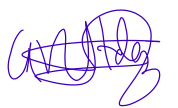
\includegraphics[height=1.2cm]{Graphics/signatures/firma_amanda.png}} \\[1cm]
Lic. Juan Miguel Pérez & \raisebox{-0.4cm}{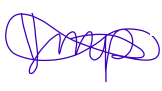
\includegraphics[height=1.2cm]{Graphics/signatures/firma_juan_miguel.png}} \\[1cm]
DraC. Marta L. Baguer & \raisebox{-0.4cm}{
\includegraphics[height=1.2cm]{Graphics/signatures/firma_marta.jpg}} \\
\end{tabular}

\end{opinion}